\section{Using MARS}
Currently, MARS v1.0 is used with EDISON system. However, MARS is a general purpose network services that can be integrated with other systems through the REST API. In this section we describe all MARS endpoints grouped by each service. 
A sample network, see Figure~\ref{fig:sample-network}, is used in the illustrative examples in the API document. Each node has eight attributes (id integer, degree integer, betweeness\_centrality real, clustering real, load\_centrality real, node\_clique\_number integer, closeness\_centrality real, clustering\_galib real).


\noindent \textbf{Notes}:
\begin{itemize}
\item All the possible responses are listed under 'Responses' for each method. Only one of them is issued per request server.
\item All responses are in JSON format.
\item Some of requests parameters are optional and have default value.
\item Host name and port number can be changed in mars.config file. 
\end{itemize}



\begin{figure}[H]
\centering
%\label{fig:ebola-kshell-not-effective}
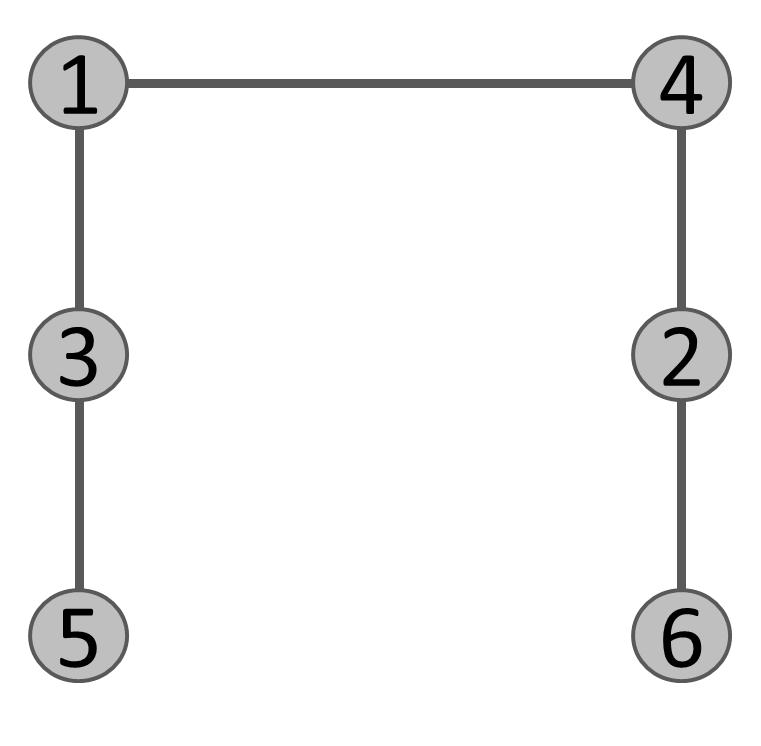
\includegraphics[trim = 0.0in 0.0in 0.0in 0.0in,scale=0.55]{sample-network.png}
\caption{
Sample network used in the illustrative examples. The network consists of six nodes. All the nodes have degree equals to two, except nodes 5 and 6 which have degree equals to one.
}     

 
\label{fig:sample-network}
\end{figure}
\subsection{MARS API Document}

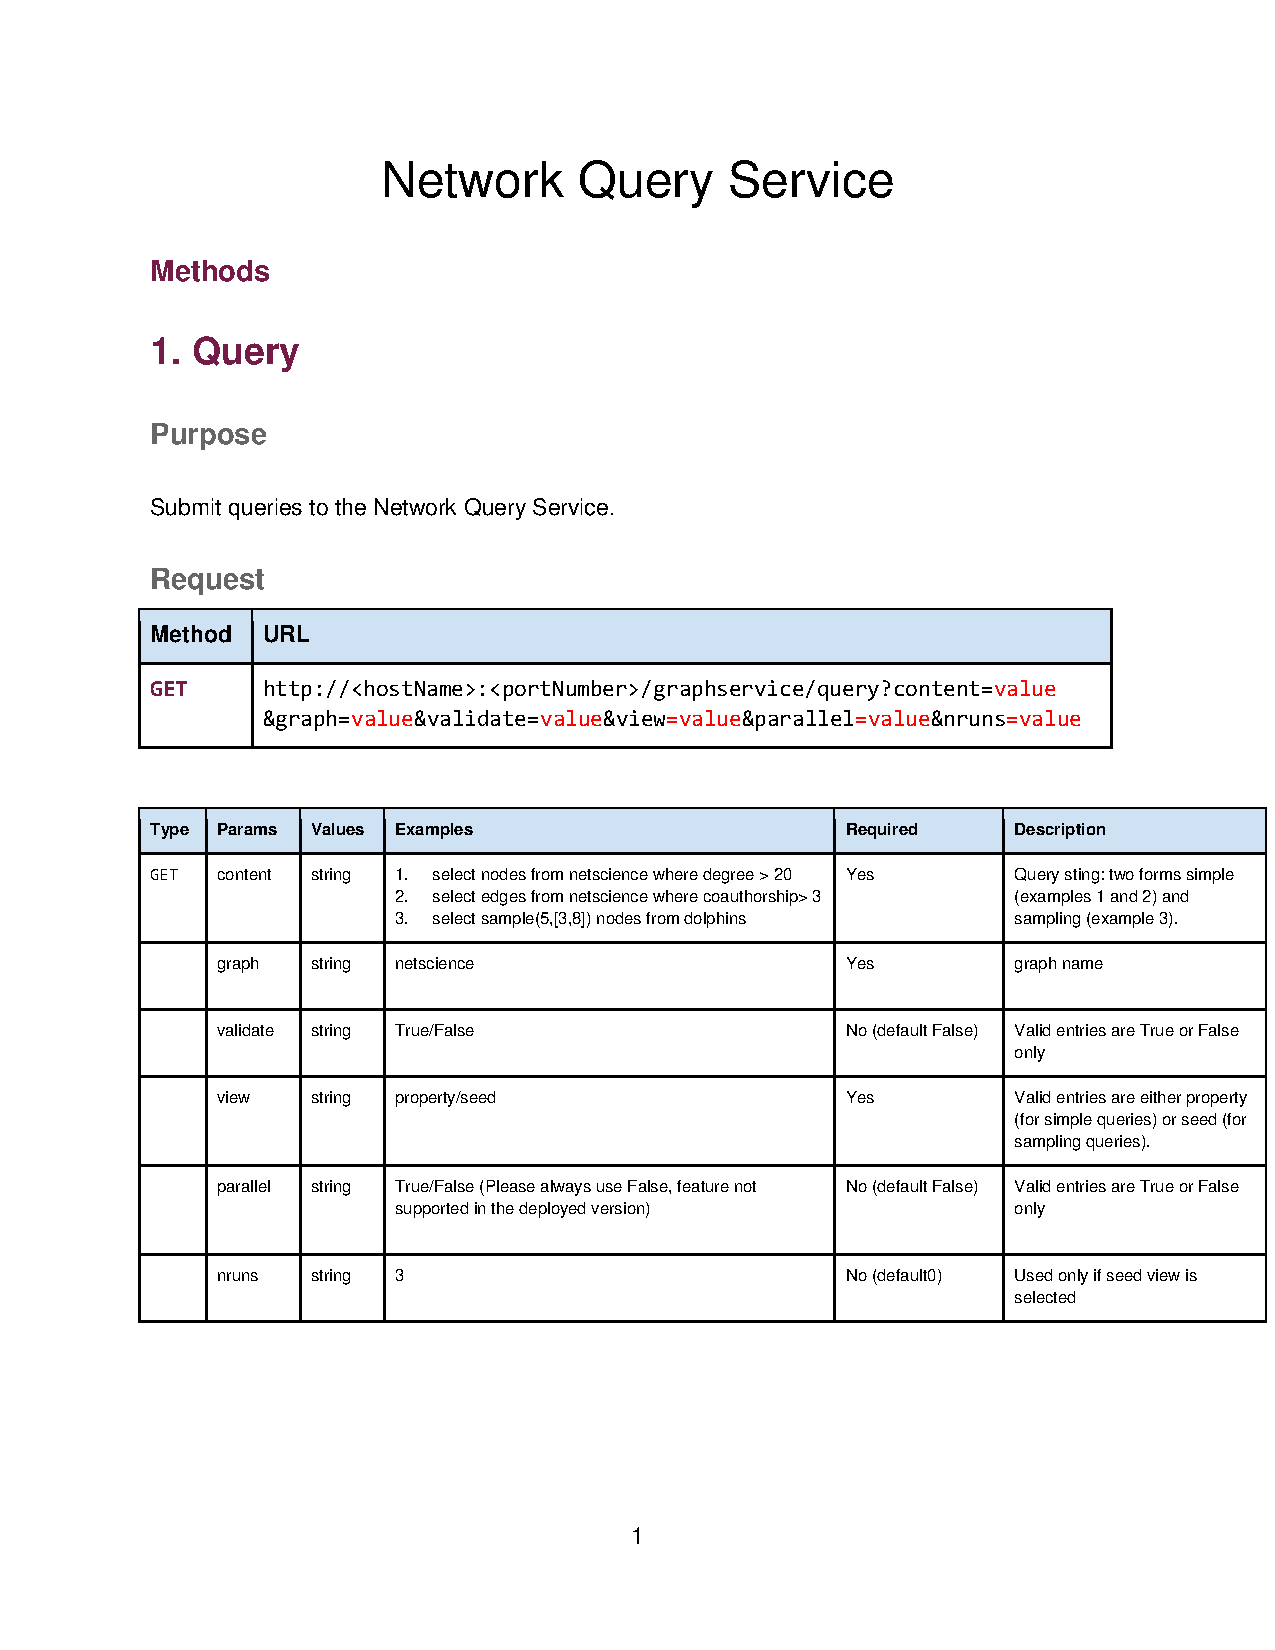
\includepdf[pages={-}]{mars_api.pdf}